\chapter{Function of Random Variable}

\section{Problem Statement} 

\textit{Show that the sum of two independent identically distributed exponential random variables is a gamma distribution.} \\


Let X and Y be two independent identically distributed exponential random variables with $\lambda=0.15$ \\
Let Z = X + Y \\
Find the pdf of Z, and obtain its parameters by independently generating 1000 values for X and Y

\section{Analytical Solution} 

\begin{align*} 
X &\sim Exp[\lambda]		 &		0 \le X \le \infty \\ 
Y &\sim Exp[\lambda]		 &		0 \le Y \le \infty \\ 
Z &= X + Y		 		&		%0 \le Z \le \infty
\end{align*}
where, \\
X~and~Y~are~independent


\begin{align*} 
X &= Z - Y		 &		0 \le X \le Z \\
\end{align*}

The distribution function for Z, 
\begin{align*} 
f_{Z}(z)	=	\int_{-\infty}^{\infty} f_{X}(x) ~ f_{Y}(z-x) ~ dx \\
			=	\int_{0}^{z} \lambda ~ e^{-\lambda~x} ~ \lambda ~ e^{-\lambda~(z-x)} ~ dx \\
			= \lambda ^2	~	z	~	e^{-\lambda z}
\end{align*}
which is a gamma distribution \\
\begin{align*} 
f_Z(z)&=\frac{\nu(\nu z)^{a-1}}{\Gamma(a)} ~ e^{-\nu z} &  z \ge 0 \\
&=0 	& 	z < 0
\end{align*}

with $a = 2 $ and $\nu = \lambda$

\section{Numerical Solution} 
The problem is solved numerically by independently generating 1000 exponential random variables for X and Y with $\lambda = 0.15$  using Python-based \textit{scipy.stats} library.

\textbf{Obtained parameters for Z are a = 2.0114 and $\nu$ = 0.1482 \\}
The histogram, and PDF are plotted for X, Y and Z as below. \\

\begin{figure}
	\centering
	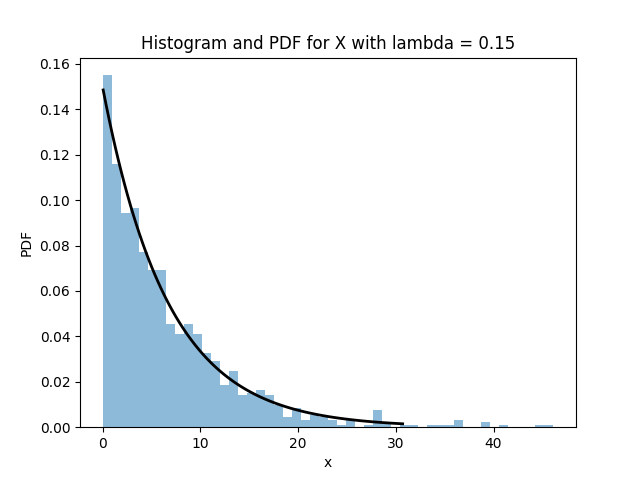
\includegraphics[width=0.9\linewidth]{Figures/Chapter1/Figure_1}
	\caption{Histogram and PDF for X with $\lambda$ = 0.15}
	\label{fig:figure1}
\end{figure}

\begin{figure}
	\centering
	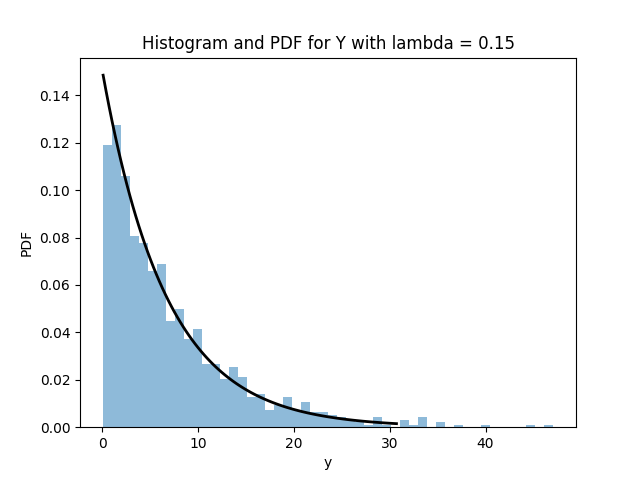
\includegraphics[width=0.9\linewidth]{Figures/Chapter1/Figure_2}
	\caption{Histogram and PDF for Y with $\lambda$ = 0.15}
	\label{fig:figure2}
\end{figure}


\begin{figure}[H]
	\centering
	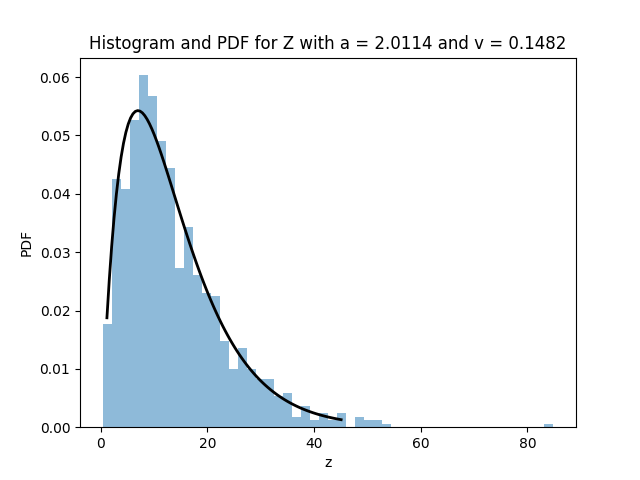
\includegraphics[width=0.9\linewidth]{Figures/Chapter1/Figure_3}
	\caption{Histogram and PDF for Z with a = 2.0114 and $\nu$ = 0.1482}
	\label{fig:figure3}
\end{figure}

The \textit{Python} code used for this computation is given in \ref{Chap:appendix:1}{ Appendix} \\
The source codes are made available in \href{https://github.com/ajmalbabums/ce605assignments.git}{github.com/ajmalbabums/ce605assignments}